\documentclass{beamer}
\usepackage{graphicx}
\usepackage{xeCJK}
\setCJKmainfont{WenQuanYi Zen Hei}
\usetheme{Frankfurt}
\useinnertheme{circles}
%\setbeamercolor{normal text}{bg=yellow!80!green} %background color using xcolor
%\setbeamertemplate{navigation symbols}{}  %no navigation bar
\hypersetup{colorlinks=true,linkcolor=red}
\begin{document}
%%-----------------------------------
{
%\setbeamertemplate{background canvas}{
\includegraphics[width=\paperwidth,height=\paperheight]{model.jpg}}
\begin{frame}
    \title{文献阅读:{\color{red}{A high-resolution map of human evolutionary constraint using 29 mammals}}}
    \author{元件注释}
    \institute{BGI-RD\\深圳}
    \maketitle
\end{frame}
}

\begin{frame}{Outline}                       %contents only page !
\tableofcontents
\end{frame}
%%-------------------------
\begin{frame}{研究背景}
%如果控制颜色的花括号不空行的话会被latex当成是标题的次标题,这时使不能加双斜线断行的,空行之后就没有误会,可以断行了

{\color{red}{已知:}}\\
人类基因组中编码部分约1.5\%,HMRD表明5\%受到purifying selection,其中又~3.5\%是非编码元件,可能与基因调控相关。\\
{\color{red}{已有研究:}}
\begin{itemize}				
\item HMRD:human-mouse-rat-dog
\item Sipel:vertebrate 
\end{itemize}
之前的比较基因组研究确定了这部分区域大体含量,但是不能检测到具体的constraint element,因为分辨率不够,所以之前的工作只是针对5\%中最保守的top 5\%。
\end{frame}

\begin{frame}{本文工作}
自2005年为29哺乳动物测序,以人类基因组做参考,确定高分辨率的map,希望找到并细致分析保守元件。
\begin{itemize}
\item 肯定了之前关于保守元件约占总量5\%的估计
\item 确定了覆盖4.2\%序列的保守元件,利用多种证据确定了其中60\%是功能相关的
	\begin{itemize}
	\item	protein-coding 
	\item RNA
	\item 调控区和chromatin roles
	\end{itemize}
\item 提供了exaptation 和加速进化的证据
\end{itemize}
{\color{red}{Expation}}:在进化过程中一些特征改变了最初的功能 -by Gould\\
$$http://en.wikipedia.org/wiki/Exaptation$$								
\end{frame}
					
\begin{frame}{sequencing,asembly and alignment}
shotgun深度:
\begin{itemize}
\item 7-fold:9  species previously described
\item 2-fold:20 species first reported
\end{itemize}
20species 质量统计:\\
\begin{itemize}
\item contig size $N50_c$ :2.8kb 
\item scaffold size $N50_s$ :51.8kb 
\item 96\% had quality score $Q_{20}$,corresponding to a <1\% error rate
\end{itemize}
\end{frame}

\begin{frame}{sequencing,asembly and alignment}
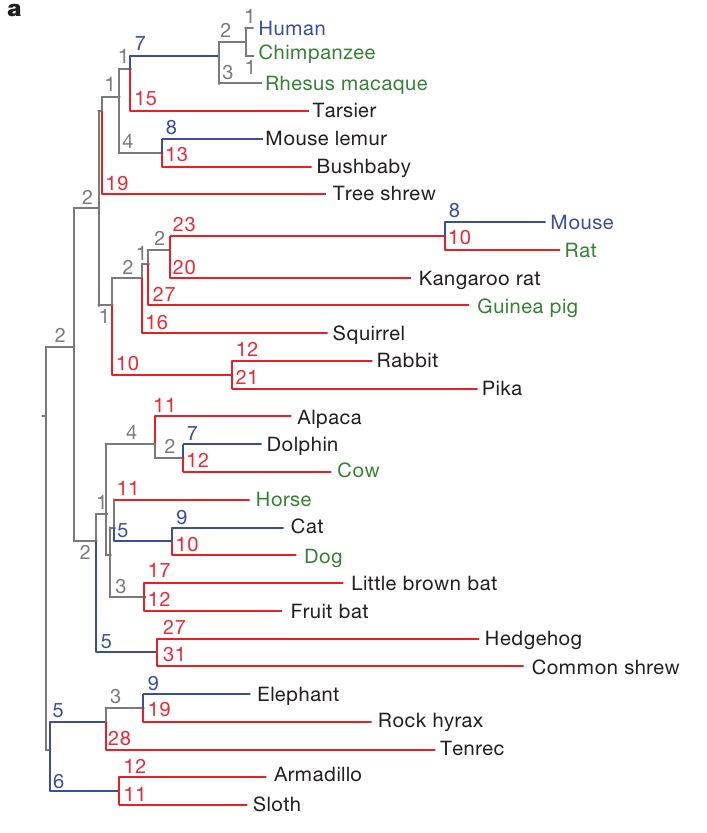
\includegraphics[width=8cm,angle=-90]{../clade.png}
\end{frame}

\begin{frame}{sequencing,asembly and alignment}
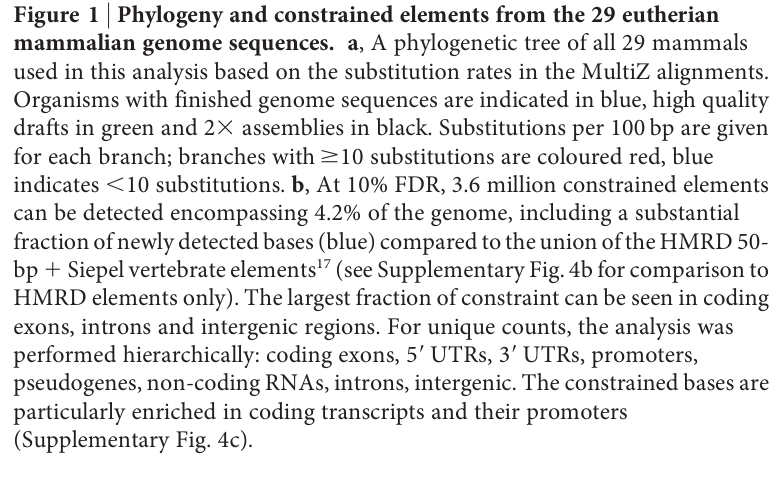
\includegraphics[width=10cm]{../clade_notes.png}
\end{frame}

\begin{frame}{sequencing,asembly and alignment}
增加了物种间的差异,枝长显著增加。
\begin{itemize}
\item HMRD:0.68 substitution per site
\item 20Ma:4.5  substitution per site
\end{itemize}
检验保守元件的能力主要取决于进化树的总枝长:the power to detect constrained elements depends largely on the total branch length of the phylogenetic tree connection the species.\\
Cooper,G.M, {\color{red}{A quantitive estimates of sequence divergence for comparative analysis of mammaliang genomes}}
\end{frame}

\begin{frame}{multiz结果}
保守程度不同的元件类型有不同的比对层数\\
with a branch length of 4.3 substitutions per site:
\begin{itemize}
\item  20.9 at protein-coding positions in the human genomen 
\item  23.9 at the top 5\% HMRD-conserved non-coding positions
\end{itemize}
with a branch length of 2.9 substitutions per site:
\begin{itemize}
\item 17.1 at whole-genome average 
\item 可能的原因是在对whole-genome 做multiz时对非编码区的large deletion ???{\color{red}{这里需要看补充材料}}
\end{itemize}
\begin{itemize}
\item 11.4 at ancestral repeats
\item 与非功能区域的重复序列相同
\end{itemize}
\end{frame}

\begin{frame}{multiz结果}
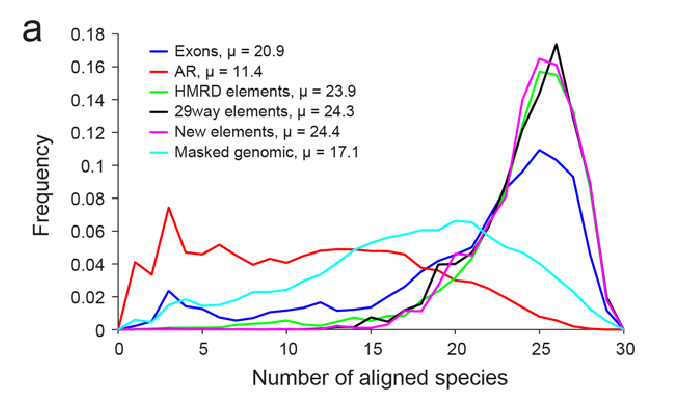
\includegraphics[width=10cm]{../numberofalignment.png}
\end{frame}


\begin{frame}{检测constrained sequence}
在整个基因组水平,用SiPhy 方法估计,保守区域约5.36\% at 50bp wondows 5.44 at 12bp windows。平均长度36bp,HMRD平均长度123bp,Sipel平均长度104bp。(图)\\
可以确定的:								
\begin{itemize}
\item 29M:
	\begin{itemize}
	\item 3.6 million elements
	\item 4.2\% at resolution of 12bp 
	\end{itemize}
\item HMRD:
	\begin{itemize}
	\item $<0.1\%$ at resolution of 12bp
	\item  $0.2\%$ at resolution of 50bp
	\end{itemize}
\item Sipel(5vertebrates):
	\begin{itemize}
	\item 4.1\% 被检测到
 	\item 其中只有45\%与29M一致,说明这次用29M检测到的很多是在哺乳动物中特有的。
	\end{itemize}
\end{itemize}	
\end{frame}

\begin{frame}{检测constrained sequence}
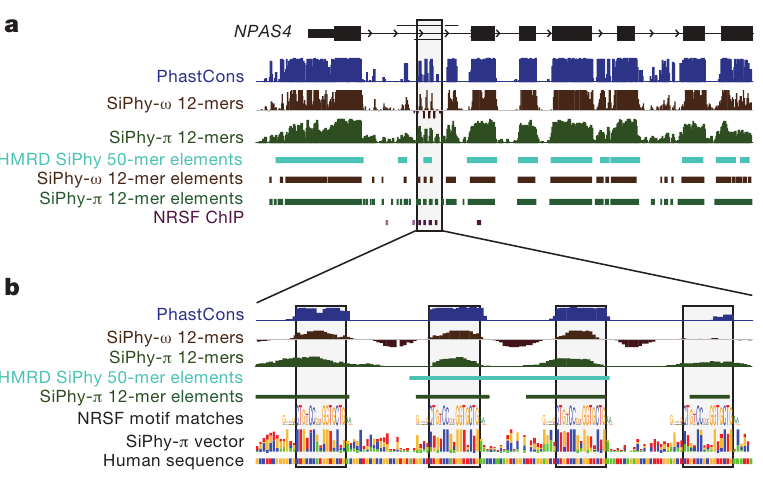
\includegraphics[width=8cm]{../NPAS4_example.png}

29M可以实现更高分辨率的保守元件检测。图中:NRSF是神经元限制沉默因子,位于NPAS4基因的启动区。之前因为对短序列的检测能力不够,没有获得完整的结构。
\end{frame}

\begin{frame}{Constrain within the human population}
We observed that the evolutionary constraint acting on the 29 ammmals is correlated with constraint within the human population,as assessed from human polymorphism data.????????
哺乳动物的保守元件在SNP中很罕见。在非编码区保守性最强的1\%元件里,snp的检出率比基因组的平均水平底1.9 fold,snp对应的等位基因也更罕见。\\
{\color{red}{SNP通常是比较活跃进化的产物}								
\begin{frame}
\begin{center}		
\begin{tabular}{c|c|c|c|c}
碱基&T&C&A&G\\
\hline
T&0&1&1.5&1.5\\
\hline
C&1&0&1&1.5\\
\hline
A&1.5&1&0&1\\
\hline
G&1.5&1.5&1&0\\
\end{tabular}
\end{center}
\end{frame}

%%----------------------------
\begin{frame}
\Huge {谢谢}
\end{frame}
%----------------------------------
\end{document}
